\documentclass[onecolumn,preprint,nosuperscriptaddress,nofootinbib,12pt,linenumbers]{revtex4-1}

%\usepackage[utf8]{inputenc}
\usepackage{slashed}
\usepackage{graphicx}
\usepackage{amssymb}
\usepackage{amssymb,latexsym}
\usepackage{amsmath,amsbsy,bbm}
\usepackage{multirow}
\usepackage[vcentermath]{youngtab}
\usepackage{nicefrac}
\usepackage[perpage]{footmisc}


\DefineFNsymbols*{lamportnostar}[math]{\dagger\ddagger\S\P\|{\dagger\dagger}{\ddagger\ddagger}}
\setfnsymbol{lamportnostar}
\renewcommand\thefootnote{\fnsymbol{footnote}}

\usepackage[dvipsnames]{xcolor} 
\newcommand{\red}[1]{\textcolor{red}{#1}} 
\newcommand{\green}[1]{\textcolor{green}{#1}} 
\newcommand{\blue}[1]{\textcolor{blue}{#1}} 

\newcommand{\eg}{\textit{e.g.}\;}
\newcommand{\ie}{\textit{i.e.}\;}
\newcommand{\eftnopi}{\mbox{EFT$(\not \! \pi)$}}
\newcommand{\ve}[1]{\ensuremath{\boldsymbol{#1}}}
\newcommand{\ls}{\ve{L}\cdot\ve{S}}
\newcommand{\be}{\begin{equation}}
\newcommand{\ee}{\end{equation}}
\newcommand{\la}{\label}

\begin{document}

\title{JLM-Machester}
\author{J K L C M S}
\date{October 2018}


\maketitle


\section{Overlook}
\begin{enumerate}
    \item numerical evidence (3,4,5, and 6-bodies) for the non-existence of shallow P-wave poles via momentum-independent contact interactions;
    \item gerneralization to the conjecture that $\slashed{\exists}$ contact theory that yields a stable
    A-{\bf fermion} system with respect to breakup into any A-n-fermion structure;
    \begin{enumerate}
        \item rigorous, analytical pair-counting arguments
        \item \red{single-particle, shell-modell prove of the vanishing P-wave-state matrix element of momentum-independent
        contact interactions for an {\bf A-fermion} system;}
        \item \red{on the scaling of the interaction which is induced by the statistics of the particles, only, on the
        number of interacting particles;} 
        \item supporting numerical evidence;
    \end{enumerate}
    \item \blue{is a perturbative treatment of P-dependent interactions enough to overcome this limitation?
     at LO the above precludes \eftnopi; is pionless EFT a viable candidate, nevertheless at NLO?
        No, because its perturbative character does not allow for the modification of potentially exisitng far-away-from-threshold poles}
    \item consequence for a {\bf nuclear} EFT which is useful for the description of P-wave systems;
    operator structure {\bf and} renormalization conditions.
\end{enumerate}


\section{Introduction}
Historical overview of pionless in S-wave / P-wave up to cluster - $^5$He.
Application in Lattice.
Explain troubles in 16O.

Needing to extend to P-wave systems. (define briefly what a p-wave system is).
Explain that Petrov already tried that but with different formalism and only 2 fermions and we extend it.

\section{Pionless theory at LO}
The formulation of a nuclear interaction theory which comprises solely neutron and proton degrees of
freedom in combination with the effective field theory formalism was shown useful in describing
processes in which nucleons exchange momenta comparable in magnitude to those which dominate
the deuteron bound state, \ie, $k_d\sim\sqrt{m_NB_d}$. The quantum-field-theoretical aspect is retained
despite the non-relativistic character of the nucleons through the relation of the defining Lagrangian
with the amplitude pertaining to the observable of interest. This prescription employs the
Lehmann-Symanzik-Zimmermann reduction formula (Peskin eqs. 4.90/4.103 ch.7), which demands the
definition of asymptotic states, \eg, for Compton scattering on a deuteron at leading order
$\vert\mathcal{IN}\rangle=\vert n,p,T=0,S=1,B_d\sim2.2~\text{MeV},\gamma,k_\gamma\rangle$


Usual explanation about Pionless <-> ERE and LO structure
Needing to have LO non perturbative treatment.
We use cut-off regularization
Thomas collapse
Effective range treatment (Wigner bound)

\subsection{Pole shifts at higher order}
\blue{(Lorenzo)} Here we should explain that also including higher order of the 
theory we can not move the pole structure but only perturb the T-matrix amplitude.

\subsection{A=4,5,6 pole structure at LO}
Here we need the phase shift calculation for the many body systems to show what for the physical parameters they dont have 



\section{Extension to general \eftnopi}
Explain that we want to extend the formalism to general S-wave poles,
ant then apply the formalism to P-wave systems.
We want to show that there exist the possibility to design a "un-physical" \eftnopi at LO
that creates shallow-poles/bound-states in P-wave systems.
If we can not find in any way, since the impossibility to move poles including next orders without iterating them, 
we have to iterate p waves.

\subsection{$^3$n and $^4$n}
\blue{(Lorenzo)} 


\begin{figure}[h] 
\centering 
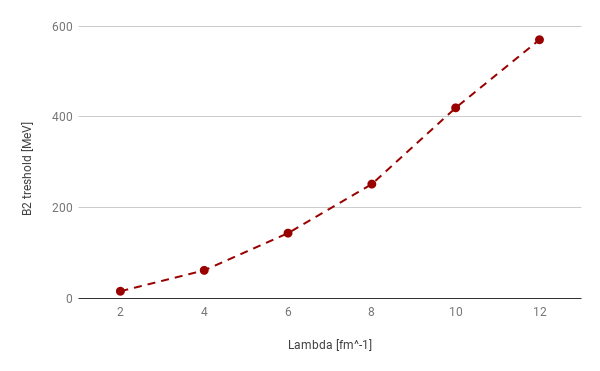
\includegraphics[width=0.8\textwidth]{./2b_3b_treshold} 
\label{fig:nnn_treshold}
\caption{Two-body binding energy at which the three body system becomes bound in function of the cutoff.} 
\end{figure} 

The $^3$n and $^4$n systems are good representative of p-wave systems with relative angular momentum J=0$^+$ and 1$^-$.
It is known from atomic physics that those systems are unstable with respect to the dibarion-n and dibarion-dibarion decay for any contact interaction. It is however interesting to translate the results in pionless formalism, where a cutoff regularization is introduced.
To show that no contact theory, regardless the strength of the interaction, can not bind three and four two-species fermions, we study the behaviour of such systems with the cutoff and effective parameters. Should be noticed that three body interaction in s-wave vanishes in those systems, however Thomas collapse can not happen either.
For simplicity, we also drop any spin-dependence in the interaction, hence only one LEC remains as parameter of the theory. 

Studying the $^2$n and $^3$n energy increasing the strength of the interaction for finite cutoff, we find first the appearance of a two-body bound state, then also the three body system becomes bound and stable. 
Increasing the cutoff, the threshold energy for which the two and three body systems are degenerate \footnote{ i.e. increasing further the binding would stabilize the three body one} increases (see figure \ref{fig:nnn_treshold}).
This stable state represents a pole in the three body T-matrix, which is deeper, in the imaginary momentum, than the $^2$n+n one.
However, from the increasing threshold energy with respect to the cutoff running can be seen that such pole fades to infinity in the contact limit. Therefore, it is not essential and it does not represent a real binding of the theory.
This is equivalent to state that in the contact limit and for each finite coupling, the $^2$n+n scattering system is less energetic than the $^3$n system, destabilizing it. 
This is in agreement with the impossibility of binding three fermion system in atomic physics described by \cite{Petrov}.

We find the same in the dibarion-dibarion.

Analyzing this piece of information with the impossibility to swap position of \eftnopi ploes adding subleading perturbative interactions, makes the description of stable bound states in $^3$n impossible with ordinary EFT description.










\subsection{$^5$He and $^6$He}
Show the same thing in 5 and 6 body systems.



\section{Extension to larger systems}
Show naive triplet counting and say that in principle if you reduce three body force you can bind manybody systems without affecting the few body ones.
Argue that almost all the triplets are non "genuine" so the number of pairs and triplets are proportional in S-wave systems.

\subsection{Potential pole vanishing and antisymmetrization contribution}
Show that the potential matrix elements between the antisymmetric components vanish.
What antysymmetrization does?

\section{Conclusions}
---
Show paper that says that can not be used dimensional regularization.

\newpage

\section*{appendix}

The interaction parameters specified in table~\ref{tab.testlec}~are tuned such that a
three-nucleon state is bound equally deep with respect to its lowest breakup threshold as
the two-body states.

This potential does not stabilize the three-neutron system. If the two-body parameter $C^\Lambda$
is tuned to increase the attraction, the three neutrons eventually form a stable system. This
bound state, for $\lim_{\Lambda\to\infty}$, is a consequence of a contact interaction
between $n^\upharpoonright$ and $n^\downharpoonright$, which induces an effective attraction
between the probe and the cluster. {\bf ECCE}, the bound state emerges in $J^\pi=\frac{1}{2}^-$, \ie,
quantum numbers which resemble the fact that the probe resides in an excited ``shell'' and does
not form a spatially totally symmetric wave function.

\begin{table*}[h!]\la{tab.testlec}
\setlength{\tabcolsep}{20pt}
\renewcommand{\arraystretch}{1.1}
\begin{center}
\begin{tabular}{ c c c }
 $\Lambda$~[fm$^{-1}$]   &   $C^\Lambda$~[MeV]     &    $D^\Lambda$~[MeV] \\\hline
2            &   -132.39852  & 220.98176 \\
4            &   -484.95744  & 1026.2260 \\
6            &   -1063.3194  & 2622.8573 \\
10           &   -2882.4086  & 7442.2430 \\
\end{tabular}
\end{center}
\caption{\small Interaction parameters (see Eq.~\eqref{eq.int-lo}, 2NI {\it attractive},
3NI {\it repulsive} $\forall\Lambda$) yielding a 2-nucleon bound state with $B(2)~\approx 1~$MeV and a
neutron-proton-neutron $J^\pi=\frac{1}{2}^+$ 3-body state
with $B(3)\approx~2~$MeV at $m_\pi=140~$MeV. 
}
\end{table*}

\begin{equation}\label{eq.int-lo}
    V(\ve{r}_{ij})=\sum_{i<j}C^\Lambda e^{-\frac{\Lambda^2}{4}\ve{r}_{ij}^2}+
D^\Lambda \sum_\text{\scriptsize cyc} e^{-\frac{\Lambda^2}{4}\left(\ve{r}_{ij}^2+\ve{r}_{ik}^2\right)} \hat{P}^S_{\nicefrac{1}{2}}
\end{equation}

The three-body force, which is repulsive (here), ensures that the ``bosonic''
\footnote{We use a 
$[s_1\otimes s_2]^0\otimes s_3]^{\nicefrac{1}{2}}$
spin-coupling scheme, \ie, compared with 
${}^3$H, no $[s_1\otimes s_2]^{\red{1}}\otimes s_3]^{\nicefrac{1}{2}}$
structure.}
three-body system is
bound by about the same amount as the two-body systems are. Na\"ively, this should produce systems
of similar spatial extent. Thereby, the enhanced attraction of the probe to the cluster with the number
of constituent bosons bound within the latter should be dominated by the increased number of allowed
interaction and not by an enhanced probability to find the probe within the core. For the larger
target cluster, one considers the shallow member of the pair of $A+1$-meres which accompanies a
preceeding $A$-body cluster ($A=3$ corresponds to a shallow Efimov trimer and the correlated pair
of tetrameres contains a deeply bound state and a shallow state).

\begin{table*}[h!]\la{tab.critlec}
\setlength{\tabcolsep}{10pt}
\renewcommand{\arraystretch}{1.1}
\begin{center}
\begin{tabular}{ c c c c c c}
 $\Lambda$~[fm$^{-1}$]   &   $C^\Lambda$~[MeV]     &    $\eta_c$  & $B_c(ab,~{}^1S_0)$~[MeV] & $B_c(abc,~\frac{1}{2}^+)$~[MeV] & $B(aba,~\frac{1}{2}^-)$~[MeV]\\ \hline
2            &   -132.39852  & 2.87 & 88   & 161  & 89   \\
4            &   -484.95744  & 3.4  & 416  & 705  & 419  \\
6            &   -1063.3194  & 3.9  & 1169 & 1886 & 1194 \\
10           &   -2882.4086  & 4.3  & 3728 & 6140 & 3950 \\
\end{tabular}
\end{center}
\caption{\small Enhancement factor for the 2NI, s. t., $C^\Lambda\to\eta_c\,C^\Lambda$ in
Eq.~\eqref{eq.int-lo} yields the respective 2- and 3-body binding energies (${}^1S_0$-dineutron:
$B_c(ab,~{}^1S_0)$, ${}^1S_0$-$p$-triton: $B_c(abc,~\frac{1}{2}^+)$, ${}^1S_0$-$n$-trineutron:
$B(aba,~\frac{1}{2}^-)$). 
}
\end{table*}

\paragraph*{On table~\ref{tab.critlec}} We conculde, 
\begin{equation}\label{eq.b2limit}
    \lim\limits_{\Lambda\to\infty}B_c(ab)=\infty
\end{equation}
, \ie, a contact interaction cannot stabilize the $aba$ system.

\newpage
\bibliographystyle{unsrt}
\bibliography{Thebibliography.bib}
\end{document}
